%\documentstyle[10pt,twoside]{article}
%\documentstyle[twoside]{article}
\documentclass[twoside]{article}
\setlength{\oddsidemargin}{0.25 in}
\setlength{\evensidemargin}{-0.25 in}
\setlength{\topmargin}{-0.6 in}
\setlength{\textwidth}{6.5 in}
\setlength{\textheight}{8.5 in}
\setlength{\headsep}{0.75 in}
\setlength{\parindent}{0 in}
\setlength{\parskip}{0.1 in}

\usepackage{graphicx}
\usepackage{url}

%
% The following commands sets up the lecnum (lecture number)
% counter and make various numbering schemes work relative
% to the lecture number.
%
\newcounter{lecnum}
\renewcommand{\thepage}{\thelecnum-\arabic{page}}
\renewcommand{\thesection}{\thelecnum.\arabic{section}}
\renewcommand{\theequation}{\thelecnum.\arabic{equation}}
\renewcommand{\thefigure}{\thelecnum.\arabic{figure}}
\renewcommand{\thetable}{\thelecnum.\arabic{table}}
\newcommand{\dnl}{\mbox{}\par}

%
% The following macro is used to generate the header.
%
\newcommand{\lecture}[4]{
   \pagestyle{myheadings}
   \thispagestyle{plain}
   \newpage
   \setcounter{lecnum}{#1}
   \setcounter{page}{1}
   \noindent
   \begin{center}
   \framebox{
      \vbox{\vspace{2mm}
    \hbox to 6.28in { {\bf CMPSCI~677~~~Distributed and Operating Systems
                        \hfill Spring 2019} }
       \vspace{4mm}
       \hbox to 6.28in { {\Large \hfill Lecture #1: #2  \hfill} }
       \vspace{2mm}
       \hbox to 6.28in { {\it Lecturer: #3 \hfill Scribe: #4} }
      \vspace{2mm}}
   }
   \end{center}
   \markboth{Lecture #1: #2}{Lecture #1: #2}
   \vspace*{4mm}
}

%
% Convention for citations is authors' initials followed by the year.
% For example, to cite a paper by Leighton and Maggs you would type
% \cite{LM89}, and to cite a paper by Strassen you would type \cite{S69}.
% (To avoid bibliography problems, for now we redefine the \cite command.)
%
\renewcommand{\cite}[1]{[#1]}

% \input{epsf}

%Use this command for a figure; it puts a figure in wherever you want it.
%usage: \fig{NUMBER}{FIGURE-SIZE}{CAPTION}{FILENAME}
\newcommand{\fig}[4]{
            %\vspace{0.2 in}
            \centerline{\includegraphics[scale=#2]{#4}}
            \begin{center}
            Figure \thelecnum.#1:~#3
            \end{center}
    }

% Use these for theorems, lemmas, proofs, etc.
\newtheorem{theorem}{Theorem}[lecnum]
\newtheorem{lemma}[theorem]{Lemma}
\newtheorem{proposition}[theorem]{Proposition}
\newtheorem{claim}[theorem]{Claim}
\newtheorem{corollary}[theorem]{Corollary}
\newtheorem{definition}[theorem]{Definition}
\newenvironment{proof}{{\bf Proof:}}{\hfill\rule{2mm}{2mm}}

% Some useful equation alignment commands, borrowed from TeX
\makeatletter
\def\eqalign#1{\,\vcenter{\openup\jot\m@th
  \ialign{\strut\hfil$\displaystyle{##}$&$\displaystyle{{}##}$\hfil
      \crcr#1\crcr}}\,}
\def\eqalignno#1{\displ@y \tabskip\@centering
  \halign to\displaywidth{\hfil$\displaystyle{##}$\tabskip\z@skip
    &$\displaystyle{{}##}$\hfil\tabskip\@centering
    &\llap{$##$}\tabskip\z@skip\crcr
    #1\crcr}}
\def\leqalignno#1{\displ@y \tabskip\@centering
  \halign to\displaywidth{\hfil$\displaystyle{##}$\tabskip\z@skip
    &$\displaystyle{{}##}$\hfil\tabskip\@centering
    &\kern-\displaywidth\rlap{$##$}\tabskip\displaywidth\crcr
    #1\crcr}}
\makeatother

% **** IF YOU WANT TO DEFINE ADDITIONAL MACROS FOR YOURSELF, PUT THEM HERE:



% Some general latex examples and examples making use of the
% macros follow.

\begin{document}

%FILL IN THE RIGHT INFO.
%\lecture{**LECTURE-NUMBER**}{**DATE**}{**LECTURER**}{**SCRIBE**}
\lecture{10}{Feb 27}{Prashant Shenoy}{\textbf{Bharath Narasimhan}}

\section{Message Oriented Communication}
Message Oriented Communication can be viewed along 2 axes: persistence (whether the system is persistent or transient); and synchronicity (whether it is synchronous or asynchronous).

\begin{description}
  \item[Persistence] : In persistent communication, messages are stored at each intermediate hop along the way until the next node is ready to take delivery of the message. It is also called a \textit{store-and-forward} based delivery paradigm. Example: Postal system (pony express), email, etc. 
  
  In transient communication, messages are buffered only for small periods of time (as long as sending/receiving applications are executing). If the message cannot be delivered or the next host is down, it is discarded. Example: General TCP/IP communication.
  
  \item[Synchronicity] : In synchronous communication. the sender blocks further operations until some sort of an acknowledgement or response is received, hence the name \textit{blocking} \textit{communication}.
  
  In asynchronous or \textit{non-blocking communication}, the sender continues execution without waiting for any acknowledgement or response. This form needs a local buffer at the sender to deal with it at a later stage. 
\end{description}

\section{Combinations - Persistence and Synchronicity}

\begin{figure}
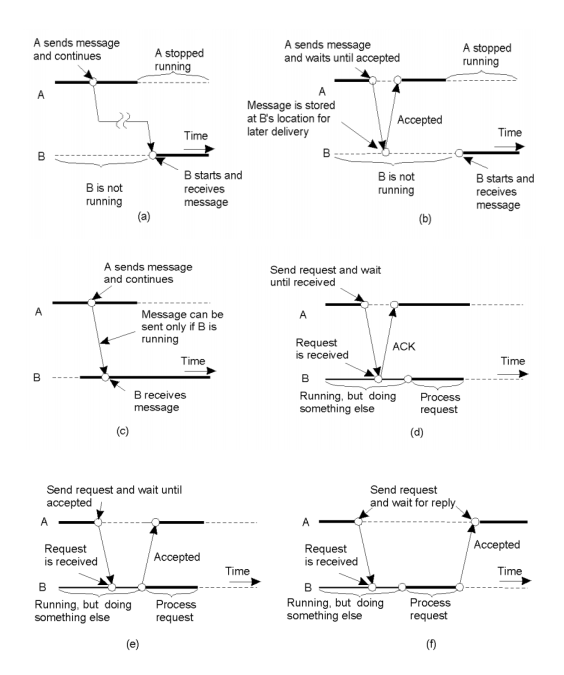
\includegraphics[width=15cm, height=18cm]{Axes.png}
% \includegraphics[width=15cm, height=6cm]{Selection_002}
% \includegraphics[width=15cm, height=6cm]{Selection_003}
\centering
\caption{Types of message-oriented communication (Although it appears as if only 4 such combinations are possible, different flavors of synchronisation acknowledgement extend it to 6 such combinations): (a) Persistent + Asynchronous (b) Persistent + Synchronous (c) Transient + Asynchronous (d) Receipt-based Transient Synchronous (e) Delivery-based Transient Synchronous (f) Response-based Transient Synchronous}
\end{figure}

\subsection{Persistent Asynchronous}
Figure 10.1 (a) gives us a time-line map for persistent asynchronous communication. A is the sender and B is the receiver. Dark line depicts execution. A sends a message and keeps executing without blocking. The message sent from A will take an arbitrary amount of time to reach B. A may or may not be running by the time the message reaches B. Disks or multiple memory queues could be used for storage at B's side. There is a guarantee that the message will eventually reach B. B receives this request and processes it then. Example: Emails can take an arbitrary amount of time to reach, and when the receiver reads the email, the sender might not even be running. 

\subsection{Persistent Synchronous}
Figure 10.1 (b) explains persistent synchronous communication. Here, A sends a message, and is then blocked (depicted by the dotted line). The acknowledgement is for receipt (not delivery/response). Because this model is persistent, the message may stay in B's queue (or in any router along the way) for an arbitrary amount of time. Example: Messaging and chat applications; Many messaging systems are persistent, and can tell us the delivery status.

\subsection{Transient Asynchronous}
Figure 10.1 (c) explains this form of communication. A sends the message and continues execution (non-blocking). B has to be running, because if it is not running the message will be discarded. Even if any router along the way is down, the message will be discarded. UDP communication is an example of transient asynchronous communication. The function $MPI\_bsend$() is an implementation of this.


\subsection{Receipt-based Transient Synchronous}
Figure 10.1 (d) explains receipt-based transient synchronous communication. A's message to B is blocking (synchronous) until an ack is received. This ack simply tells us that the message was received at the other end. It does not tell us anything about whether the process has started.

% \begin{figure}[b]
% \centering
% \end{figure}

\subsection{Delivery-based Transient Synchronous}
This is an extension of receipt-based transient synchronous communication. As shown in figure 10.1 (e), A will resume running when B takes the delivery of the message. The ack comes a little bit later than the previous method. This is essentially asynchronous RPC because from the perspective of an RPC, we are not blocking for the reply.

\subsection{Response-based Transient Synchronous}
Figure 10.1 (f) explains this type of communication. A resumes execution upon receiving a response. That is, not only has the message been delivered, but it has been processed and the ack comes back in the form of a reply. This is traditional RPC. The client is blocked for the entire duration the reply comes back.

\textbf{QUESTION} : When will the message get lost?\\
\textbf{ANSWER} : We assume that the network is not dropping messages here, just a conceptual description.

\textbf{QUESTION} : What if the server is not even running in case f) ? \\
\textbf{ANSWER} : If the server is not running, RPC will not even go to the server because it cannot bind to it. However if the server was bound to and then crashed, some form of port error would be thrown.

\section{Message Oriented Transient Communication}
Berkeley Socket Primitives, and Message-Passing Interface (MPI) are examples of message-oriented transient communication. These systems do not use on-disk queues for message storing. Below, we map the MPI primitive functions to one of the above types. MPI\_bsend simply appends the outgoing message to the local send buffer, and then keeps running. Thus, it is transient asynchronous communication. MPI\_send sends a message and waits until copied to the remote buffer. This is similar to delivery-based transient synchronous communication. MPI\_ssend waits until receipt start and MPI\_sendrecv waits for a reply, classifying each to receipt based and reply based transient synchronous communication respectively. Hence, these constructs map very well to the 6 different communication types mentioned above. MPI allows you to choose what kinds of combination of Sync communication you wish to use. It is a much richer communication system where the programmer can choose what form of communication to use from a spectrum of choices.


\section{Message Oriented Persistent Communication}
This class of communication is called Message Queuing Systems (MQS). They use on-disk buffers to ensure persistence of messages over long periods of time. Common open-source examples include Kafka, RabbitMQ, ActiveMQ, ZeroMQ, etc. An application level example for this is emails. All emails are stored on disks til delivery. The queues have names/addresses which are used to explicitly put messages into the queue. This is a form of \textit{store-and-forward} communication. Persistence neither guarantees the duration in which the message will be delivered, nor the reading of the message. It only ensures delivery. Thus, it is a loosely coupled communication. 

\begin{figure}
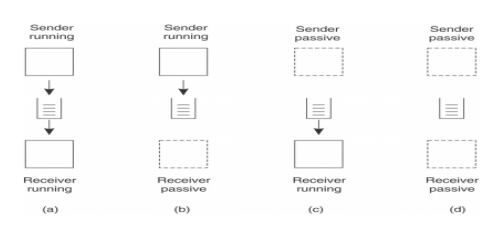
\includegraphics[width=15cm, height=6cm]{MQ.png}
\centering
\caption{Various use cases of a Message Queuing Model }
\end{figure}

Figure 10.2 explains the working of an MQS. The figure represents a series of queues(doing hop-by hop delivery) as a single abstract persistent queue. Dark boxes indicate execution, while dotted boxes indicate that the system is not running. The first case (a) is the simplest where both A and B are running, and the message is delivered immediately. 
\\In case (b) where B is not running, the message is stored at the queue and B takes delivery at a later point. Example - email.
\\ In case (c), the sender is not running when B receives the message. Example - Reading email
\\In case (d), the message is queued for an arbitrary amount of time as both A and B are passive. This is loose communication because the sender and the receiver are not participating in the communication at the same time.

The typical abstractions used in the message queuing model are \textit{get} and \textit{put}. \textit{put} allows us to insert into a specific queue. \textit{get} removes a message from the head of the queue. \textit{get} and \textit{put} are analogous to \textit{send} and \textit{receive}. There is a non-blocking \textit{poll} as well, which checks the queue for a message and  returns the message if the queue is non-empty. It is a periodic process (might lead to resource wastage). Example - email clients checking servers. \textit{notify} (also non-blocking) is an async message from the queue to the receiver notifying it of a message arrival.

\textbf{QUESTION} : For fault tolerance reasons, do we write to disk before notifying?\\ 
\textbf{ANSWER} : Will have to do that typically. 

\textbf{QUESTION} : What does \textit{poll} do exactly?\\ 
\textbf{ANSWER} : Remove message from the head of the queue without blocking.

\textbf{QUESTION} : Do poll and notify go hand-in-hand?\\ 
\textbf{ANSWER} : Both allow communications in an asynchronous manner .Still need to use put for insert, but can use get (blocking) or poll/notify (non-blocking) 

\begin{figure}
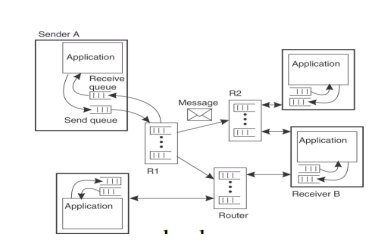
\includegraphics[width=12cm, height=6cm]{MQS.png}
\centering
\caption{General Architecture of an MQS}
\end{figure}

In a full-fledged MQS, we have MQS routers (with disk-queues) also called relays. Figure 10.3 shows an example of a typical MQS system. 
Routers in the middle provide persistent queueing. Between each hop, get/put/poll/notify can be used to get the message to it's destination. 
Commercial MQS applications are built like this, used for order processing.

Message Brokers  - Application level programs that take messages from queues and transforms it. This allows us to send messages across platforms, thus allowing interoperability. This is also used by many publish-subscribe systems, where a queue actually acts like a mailing list - having multiple receivers. The sender doesn't know who the message will be delivered to. Will revisit in Middleware systems.

IBM's Websphere MQ is a good example of MQS usage in a B2B commercial system. It works with RPC along with API's for get/put etc. (like a pub-sub system). get and put are implemented as RPC calls. Queues are persistent (as opposed to network routers which use memory buffers)


\section{Stream Oriented Communication}
Stream oriented communication is usually used in audio and video streaming.
\\\textit{Message communication} can be thought of as a request-response. In \textit{Stream communication}, you might start receiving data without it being requested. 
One aspect of stream communication is \textit{timing constraints}. 
Playback freezes if data is not delivered on time, affecting the streaming experience (as opposed to browsing, where it does not matter as much).\\
This form of communication is called \textit{isochronous communication}. If we wish to watch 30 fps,a frame needs to come in every 33 ms. This implies that the end-to-end delay cannot be arbitrary, it must have an upper bound. Stream communication is not client pull-based (like message comm.), it is server push-based. 

There are 2 kinds: live streaming and stored streaming.\\ Live streaming (Example: Video conferencing) is when both parties are live. For live streaming, the end to end delay has to be of the order of 10 ms. Typical human perception needs 150ms. \\
In Stored streaming(Example: Youtube, Netflix), one endpoint is actually a disk that stores data which the server streams. Here, the end to end delay does not matter as much, but the data rate should be a constant. 

Another way of splitting stream communication is as \textit{One-to-one} (Example: Video conference) or \textit{One-to-many} (Example: Webcast)

\subsection{Quality of Service}
QoS is a way to encode the requirements of audio and video stream.
Streaming needs a different architecture as compared to best-effort networks like the Internet that provide no guarantees.
The requirements include:
\begin{description}
\item[Bandwidth]: A HD video will need a minimum of a few Mbs per second.
\item[Maximum end-to-end delay bound]: Needs to be fixed (~100ms) to avoid playback glitches (Skype, Facetime)
\item[Jitter]: Refers to the variation in the end-to-end delay. The fluctuation in the delay is jitter. We want to minimize jitter to ensure a steady data rate.
\item[Loss]: Refers to the loss in data packets. With TCP, loss is handled using re-transmission. Fundamentally, in video streaming, retransmission may not be an option (especially for live transmissions). Late data might be as good as no data for live streaming. Time requirements can sometimes be a trigger for complex re-transmissions - hence we need to lower this.
\end{description}

\textbf{QUESTION} : What is the difference between end-to-end delay and round-trip delay? Isn't the latter just twice the former? \\
\textbf{ANSWER} : Depends on whether the network is bidirectional and what the streaming type is. Followup - RT might involve processing too? A - No, this was just considering network delays


However, networks today are best-effort. Network QoS did not go commercial, but is instructive. Some of these QoS guarantees are used in OS virtualization.
A much more exhaustive list of QoS requirements is given in figure 10.4.

\begin{figure}[t]
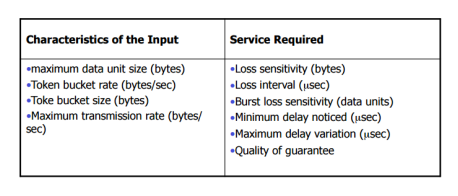
\includegraphics[scale=0.5]{qos.png}
\centering
\caption{QoS Requirements}
\end{figure}


\subsection{Token Bucket}
Token Bucket is an OS-based method of enforcing QoS. Although it is not used in audio/video streaming, it is still used in many other contexts. It is also called a Leaky Bucket Rate Regulator. It enforces a certain bandwidth, using an OS-level mechanism. In general, it deals with the bandwidth bit-rate r and burst of deviation b.

Figure 10.5 explains the mechanism. Every time a packet needs to be sent, it needs to grab a token that will be generated by the OS. The OS will generate tokens at a steady rate R. R is the bandwidth that needs to be guaranteed. Thus, we can never send at a rate higher than the specified rate R because the packet will not be able to find any token. However, the token bucket allows for some instantaneous fluctuation, captured by the second parameter - depth of the bucket. Thus, the bucket has 2 parameters : token generation rate R and instantaneous depth B. When we start off, we start with a bucket of B tokens. That is, at any time, we can instantaneously generate B packets that can grab the B tokens and go out instantly. Then, the bucket will be filled at a steady rate of R. 

Essentially, the plot of the maximum number of packets sent vs time will give us a linear plot y=mx + b, where b=B and m=R, y is the number of packets sent and x is the time. This will mean that if we generate packets at a rate greater than R, they will have to wait, as the token corresponding to the packet will not have been generated. This also specifies the upper bound.


\begin{figure}[h!]
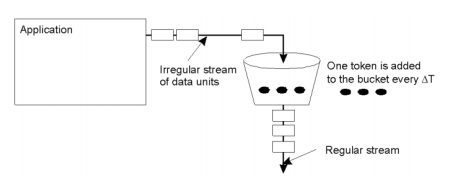
\includegraphics[scale=0.5]{leaky.png}
\centering
\caption{Leaky-Bucket model to ensure QoS}
\end{figure}

\begin{figure}[h!]
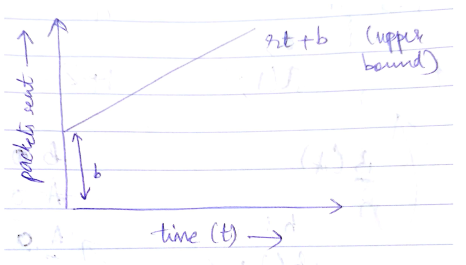
\includegraphics[scale=0.5]{leaky_graph.png}
\centering
\caption{Packets Sent v/s Time (Token Bucket)}
\end{figure}


\textbf{QUESTION} : Where does buffering happen? Does the application block if bucket is empty?\\
\textbf{ANSWER} : Happens at the Ethernet device drive; The bucket processing is invisible to the application which will keep sending.\\\\ 
\textbf{QUESTION} : This seems like an upper bound?\\
\textbf{ANSWER} : Yes it is; Use-case (2 VMs on a machine with 1GB ethernet card. Can use token bucket for each VM to allocated 500MB bandwidth to each.) Leaky bucket just a way to show how to enforce QoS. 

 
\textbf{QUESTION} : What is the advantage of burst?\\
\textbf{ANSWER} : For small amounts of time, can send faster than R (We do not want to send at R always)

\textbf{QUESTION} : When do you regenerate burst tokens?\\
\textbf{ANSWER} : There is only one kind of token first of all. Initialize bucket with $b$ tokens and every $\frac{1}{r}$ seconds, generate a token. If you generate tokens faster than you send, you will accumulate $b$ tokens.   

\subsection{Using Buffers to Enforce QoS}
We want to reduce playback glitches in video streaming. First, we will handle delay. In Figure 10.6, the x axis is time, and each numbered box is a packet. These packets will have jitter because each will arrive at a different time, even though we sent them in steady gaps. To play at a constant fps (say f), we need to play the next frame in 1/f seconds. But, after frame 1 arrives, frame 2 does not arrive in that time difference, hence resulting in a playback glitch. We might be receiving at that rate on average, but there are no guarantees. One standard method is to hold the packets in a buffer before starting playback. Hopefully, if data continues to arrive at a good rate, our buffer will always have data, and we can keep playing. However, in the figure for example, frame 8 still arrives late resulting in a playback glitch.
\begin{figure}[t]
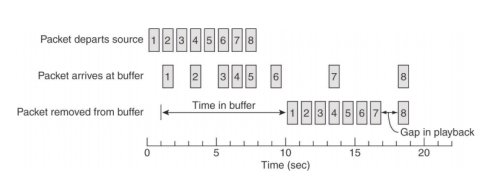
\includegraphics[scale=0.5]{playback.png}
\centering
\caption{Handling playback glitches due to delays using buffers}
\end{figure}


Figuring out the buffer size is important for video quality. (Trade-off: Too large leads to impatient user, too small leads to playback glitches)
Dynamic buffer sizes are used.

What happens when packets are dropped? The video will not look smooth anymore.
Can use FEC(Forward Error Correction) or \textit{scrambling}. The idea is to spread out the lost frames so that the perception of the problem is minimized (29 fps vs 30 fps)
\begin{figure}[t]
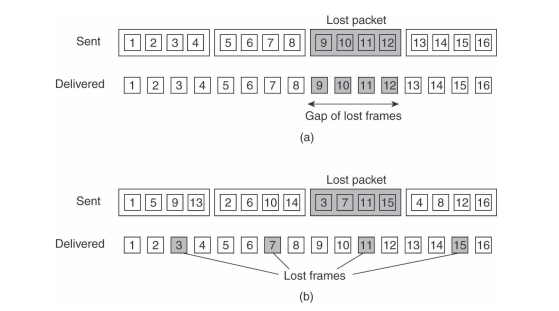
\includegraphics[scale=0.5]{playback2.png}
\centering
\caption{Handling packet losses}
\end{figure}


\subsection{HTTP Streaming}

Almost all streaming today is pull-based and happens over HTTP. The video is split into chunks which are then requested by the client. \\
\begin{figure}[t]
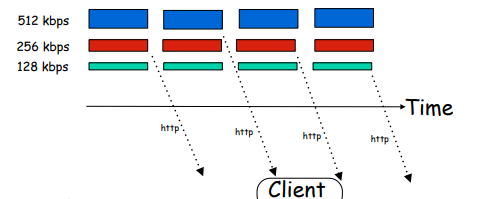
\includegraphics[scale=0.5]{dash.png}
\centering
\caption{Direct Adaptive Streaming over HTTP}
\end{figure}
\textit{DASH(Direct Adaptive Streaming over HTTP)} - Data needs to be sent at different qualities because the device at the client is not known. Intelligence is placed at the client, which requests the appropriate quality. This quality level can be lowered/raised by the client in real-time.  





\end{document}
